\documentclass[10pt,a4paper]{article}
\usepackage[margin=22mm]{geometry}
\usepackage{amsmath,amssymb,graphicx,booktabs,siunitx,caption,hyperref}
\captionsetup{font=small,labelfont=bf}
\setlength{\parskip}{4pt}\setlength{\parindent}{0pt}
\title{Why the irrigation jet makes a ring vortex in the blocked sheath\\[2pt]
\large Analytical model and check against the flow simulation}
\author{USZ sheath without internal tube, irrigation outlet in the tip}
\date{13 November 2026}
\begin{document}
\maketitle

\section*{Summary}
The irrigation leaves a \SI{1}{mm} outlet about 120 times faster than the sheath lumen needs to carry the same
flow. A fast thin jet drags the surrounding fluid along. With every side hole blocked, only the irrigation
flow itself can leave through the suction tube, so the dragged fluid has to return along the walls. That
return is the ring vortex seen in the animation. The model below gives, with no fitted constant,
\begin{itemize}\setlength\itemsep{0pt}
\item the rate at which the return flow builds up near the outlet, $8\pi\nu$ per unit length
      (simulation: the same to within 3\,\%);
\item the jet centre speed and width over the first \SI{15}{mm} (simulation: within 15\,\%);
\item the length of the loop, about \SI{32}{mm} (simulation: \SI{38}{mm});
\item the scaling of the loop length, proportional to flow rate and roughly to $1/d$.
\end{itemize}
Assembled into one flow field for a round tube (section 7), the model also gives the strength of the loop
to about 35\,\%: a peak return flow of \SI{13.6}{mL/min} against \SI{10.1}{mL/min} in the simulation, 2.4 times
the irrigation. The main thing it misses is that the lumen is oval, so the fluid returns only along the two
wide sides. An earlier estimate of \SI{57}{mL/min} from the unconfined formula ignored the walls and is withdrawn.

\section{Set-up and numbers}
\begin{figure}[h]\centering
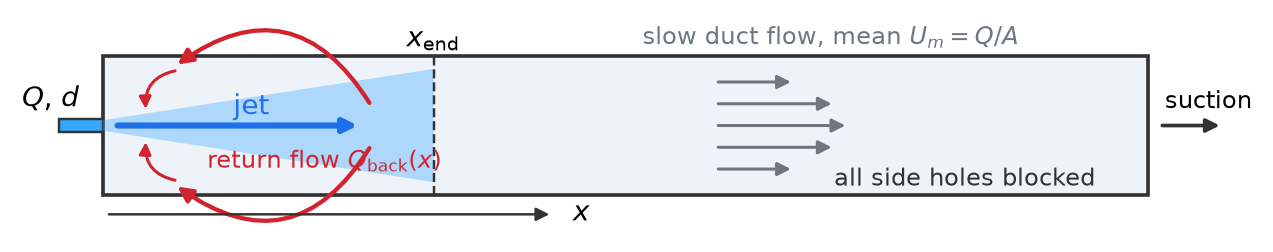
\includegraphics[width=0.92\linewidth]{fig_sketch.png}
\caption{Blocked sheath. The jet from the tip outlet (blue) entrains fluid, which returns along the walls
(red) up to $x_{\rm end}$. Beyond that the flow is a slow duct flow towards the suction tube.}
\end{figure}

Single-phase saline, $\rho=\SI{1000}{kg/m^3}$, $\nu=\SI{1e-6}{m^2/s}$, steady flow, rigid walls.
\begin{center}\begin{tabular}{llr}\toprule
Irrigation flow & $Q$ & $\SI{250}{mL/h}=\SI{4.17}{mL/min}=\SI{6.94e-8}{m^3/s}$\\
Outlet diameter & $d$ & \SI{1.0}{mm}\\
Outlet mean speed & $U_j=4Q/\pi d^2$ & \SI{88.4}{mm/s} (peak $2U_j=\SI{177}{mm/s}$)\\
Jet Reynolds number & $Re=U_jd/\nu$ & 88\\
Lumen area, equivalent radius & $A$, $R_{\rm eq}=\sqrt{A/\pi}$ & \SI{93.3}{mm^2}, \SI{5.45}{mm}\\
Lumen mean speed & $U_m=Q/A$ & \SI{0.744}{mm/s}\\
Area ratio & $A/(\pi d^2/4)$ & 119\\ \bottomrule
\end{tabular}\end{center}

\section{Momentum of the jet}
The fluid leaves the outlet tube with a parabolic profile $u=2U_j(1-4r^2/d^2)$. Its momentum flux divided
by density is
\begin{equation}
K=\int_0^{d/2}u^2\,2\pi r\,dr=\frac43\,U_j^2\,\frac{\pi d^2}{4}=\frac{16}{3\pi}\frac{Q^2}{d^2}
 =\SI{8.19e-9}{m^4/s^2}.
\end{equation}
Away from walls no force acts on the jet (the pressure is uniform, section~\ref{sec:p}), so $K$ is the same
at every distance $x$. This single conserved number fixes the whole jet.

\section{The laminar round jet (Schlichting)}
For a slender steady axisymmetric jet the boundary-layer equations are
\begin{equation}
\frac{\partial u}{\partial x}+\frac1r\frac{\partial (rv)}{\partial r}=0,\qquad
u\frac{\partial u}{\partial x}+v\frac{\partial u}{\partial r}
   =\frac{\nu}{r}\frac{\partial}{\partial r}\!\left(r\frac{\partial u}{\partial r}\right),
\qquad 2\pi\!\int_0^\infty\! u^2 r\,dr=K .
\end{equation}
With the stream function $\psi=\nu x\,F(\xi)$ and the similarity variable $\xi=a\,r/x$ they reduce to an
ordinary differential equation whose solution is $F=\xi^2/(1+\xi^2/4)$. Hence
\begin{equation}
u(x,r)=\frac{u_c(x)}{\left(1+\xi^2/4\right)^2},\qquad
\xi=\sqrt{\frac{3K}{16\pi}}\;\frac{r}{\nu x},\qquad u_c(x)=\frac{3K}{8\pi\nu x}.
\end{equation}
Two integrals of this profile matter. Using $\int_0^\infty \xi\,d\xi/(1+\xi^2/4)^4=2/3$ the momentum
flux comes out as $K$ for every $x$, as it must. Using $\int_0^\infty \xi\,d\xi/(1+\xi^2/4)^2=2$ the
volume flow carried by the jet is
\begin{equation}
Q_{\rm jet}(x)=2\pi\!\int_0^\infty\! u\,r\,dr=8\pi\nu x .\label{eq:ent}
\end{equation}
The jet therefore takes in surrounding fluid at the constant rate
$dQ_{\rm jet}/dx=8\pi\nu=\SI{1.51}{mL/min}$ per mm, whatever its momentum.

A real jet starts with finite width, so the point-source solution is shifted by a virtual origin $x_0$.
Choosing it so that the centre speed at the outlet equals the true peak $2U_j$ gives
\begin{equation}
u_c(x)=\frac{3K}{8\pi\nu\,(x+x_0)},\qquad x_0=\frac{Re\,d}{16}=\SI{5.5}{mm}.\label{eq:uc}
\end{equation}
The half-width, where $u=u_c/2$, follows from $(1+\xi^2/4)^2=2$, i.e.\ $\xi=1.287$:
\begin{equation}
r_{1/2}(x)=5.27\,\frac{\nu\,(x+x_0)}{\sqrt K}=0.0582\,(x+x_0).\label{eq:rh}
\end{equation}

\section{Why the flow must turn back}
With all holes blocked the net flow through every cross-section of the lumen equals $Q$. Split it into
the part moving towards suction and the part moving back:
\begin{equation}
Q_{\rm forward}(x)-Q_{\rm back}(x)=Q\quad\text{for every }x .
\end{equation}
The jet wants to carry $Q+8\pi\nu x$. The only source for the extra fluid is the lumen itself, so close
to the outlet
\begin{equation}
Q_{\rm back}(x)\simeq 8\pi\nu x .\label{eq:back}
\end{equation}
Fluid moves forward in the core and backward in the surrounding ring: a ring (toroidal) vortex.
The return flow already equals the whole irrigation flow at $x=Q/8\pi\nu=\SI{2.8}{mm}$.

Whether a confined jet recirculates at all is measured by the Craya--Curtet number, the ratio of the mean
duct speed to the speed scale of the jet momentum spread over the duct:
\begin{equation}
C_t\simeq\frac{U_m}{\sqrt{K/A}}=\frac{0.744}{9.37}=0.08 .
\end{equation}
Recirculation appears below $C_t\approx0.75$. This case is a factor ten inside that regime: the jet has
about 160 times more momentum than the duct flow could carry ($1/C_t^2$).

\section{Where the loop ends}
The loop ends where the jet has widened to the walls, since nothing is left to entrain. Take the edge of
the jet at $2.5\,r_{1/2}$ (speed down to 8\,\% of the centre value) and the wall at the equivalent radius:
\begin{equation}
2.5\times0.0582\,(x_{\rm end}+x_0)=R_{\rm eq}\quad\Longrightarrow\quad
x_{\rm end}=\frac{R_{\rm eq}\sqrt K}{13.2\,\nu}-x_0=37.4-5.5=\SI{32}{mm}.\label{eq:xend}
\end{equation}
The simulation gives \SI{38}{mm} (return flow below 1\,\% of $Q$). The choice of 2.5 half-widths and of a
round equivalent for the oval ribbed lumen are the two approximations here.

Substituting $K$ gives a design formula in the Reynolds number of the outlet:
\begin{equation}
\boxed{\;x_{\rm end}\simeq Re\left(0.078\,R_{\rm eq}-\frac{d}{16}\right),\qquad Re=\frac{4Q}{\pi d\,\nu}\;}
\label{eq:design}
\end{equation}
The loop length is proportional to the flow rate $Q$ and falls a little faster than $1/d$.

\section{Check against the simulation}
\begin{figure}[h]\centering
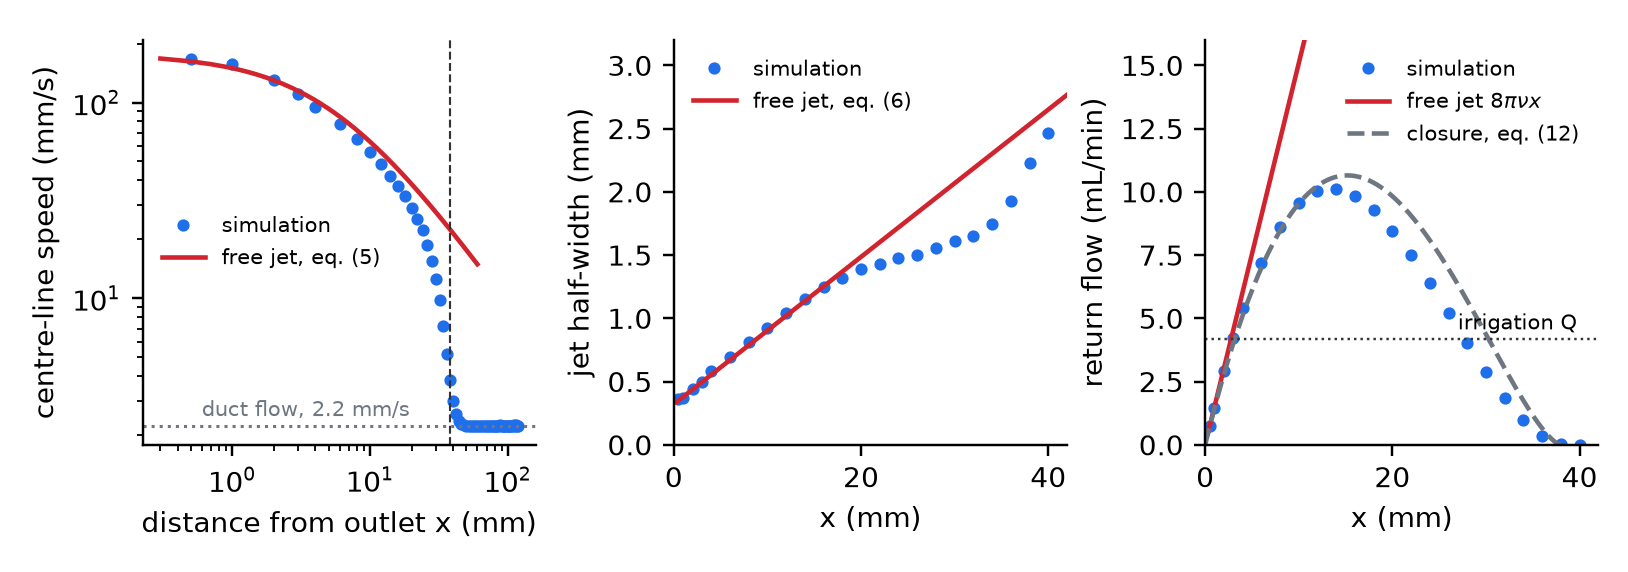
\includegraphics[width=\linewidth]{fig_jet.png}
\caption{Blocked-sheath simulation (dots, 117\,000 nodes) against the free-jet formulas (red). Left: centre-line
speed. Middle: half-width. Right: return flow through each cross-section. The dashed vertical line marks
the end of the loop in the simulation.}
\end{figure}
\begin{center}\begin{tabular}{lrr}\toprule
Quantity & Model & Simulation\\ \midrule
Build-up of return flow near the outlet (mL/min per mm) & 1.51 & 1.47\\
Centre speed at $x=\SI{10}{mm}$ (mm/s) & 63 & 56\\
Half-width at $x=\SI{10}{mm}$ (mm) & 0.90 & 0.92\\
Half-width at $x=\SI{20}{mm}$ (mm) & 1.49 & 1.39\\
Loop length $x_{\rm end}$ (mm) & 32 & 38\\
Peak return flow (mL/min) & 13.6 at \SI{17}{mm} (section 7) & 10.1 at \SI{14}{mm}\\ \bottomrule
\end{tabular}\end{center}
The entrainment rate $8\pi\nu$ is reproduced almost exactly. Beyond about \SI{12}{mm} the walls take over:
the return flow occupies a ring of limited area, it opposes the jet, and the jet slows down faster than a
free jet would. Equation \eqref{eq:back} therefore over-predicts further out. A simple closure that follows
the simulation (fitted exponent, not derived) is
\begin{equation}
Q_{\rm back}(x)\approx 8\pi\nu\,x\left(1-\frac{x}{x_{\rm end}}\right)^{3/2},\qquad
\max Q_{\rm back}\approx0.19\times8\pi\nu\,x_{\rm end}\ \text{at}\ x=0.4\,x_{\rm end}.\label{eq:closure}
\end{equation}
With $x_{\rm end}=\SI{38}{mm}$ it gives a peak of \SI{10.7}{mL/min} at \SI{15}{mm}; the simulation has
\SI{10.1}{mL/min} at \SI{14}{mm}.


\section{The whole flow field, predicted and simulated}
The pieces above can be assembled into one flow field for a round tube of radius $R_{\rm eq}$. With
$s=r^2/R_{\rm eq}^2$, $X=x+x_0$, $F(\xi)=\xi^2/(1+\xi^2/4)$ and the axial speed $u=\frac1r\,\partial\psi/\partial r$,
the stream function is
\begin{equation}
\psi(x,r)=m\,\nu X\,F(\xi)\;+\;(1-m)\,\frac{Q}{2\pi}\left(2s-s^2\right)\;-\;B(x)\left(3s^2-2s^3\right),
\qquad B=m\left[\nu X\,F(\xi_R)-\frac{Q}{2\pi}\right].
\end{equation}
The first term is the Schlichting jet, the second the duct (Poiseuille) flow, the third the return flow, with a
profile that vanishes on the axis and has no slip at the wall. $B$ is fixed by requiring the net flow
through every section to be $Q$ ($\psi=Q/2\pi$ at the wall). The weight $m(x)$ hands the jet over to the duct
flow around the predicted loop end of eq.~\eqref{eq:xend}: $m=1$ up to $0.5\,x_{\rm end}$, falling as a cosine
to $0$ at $1.5\,x_{\rm end}$. Nothing is fitted to the simulation.
\begin{figure}[h]\centering
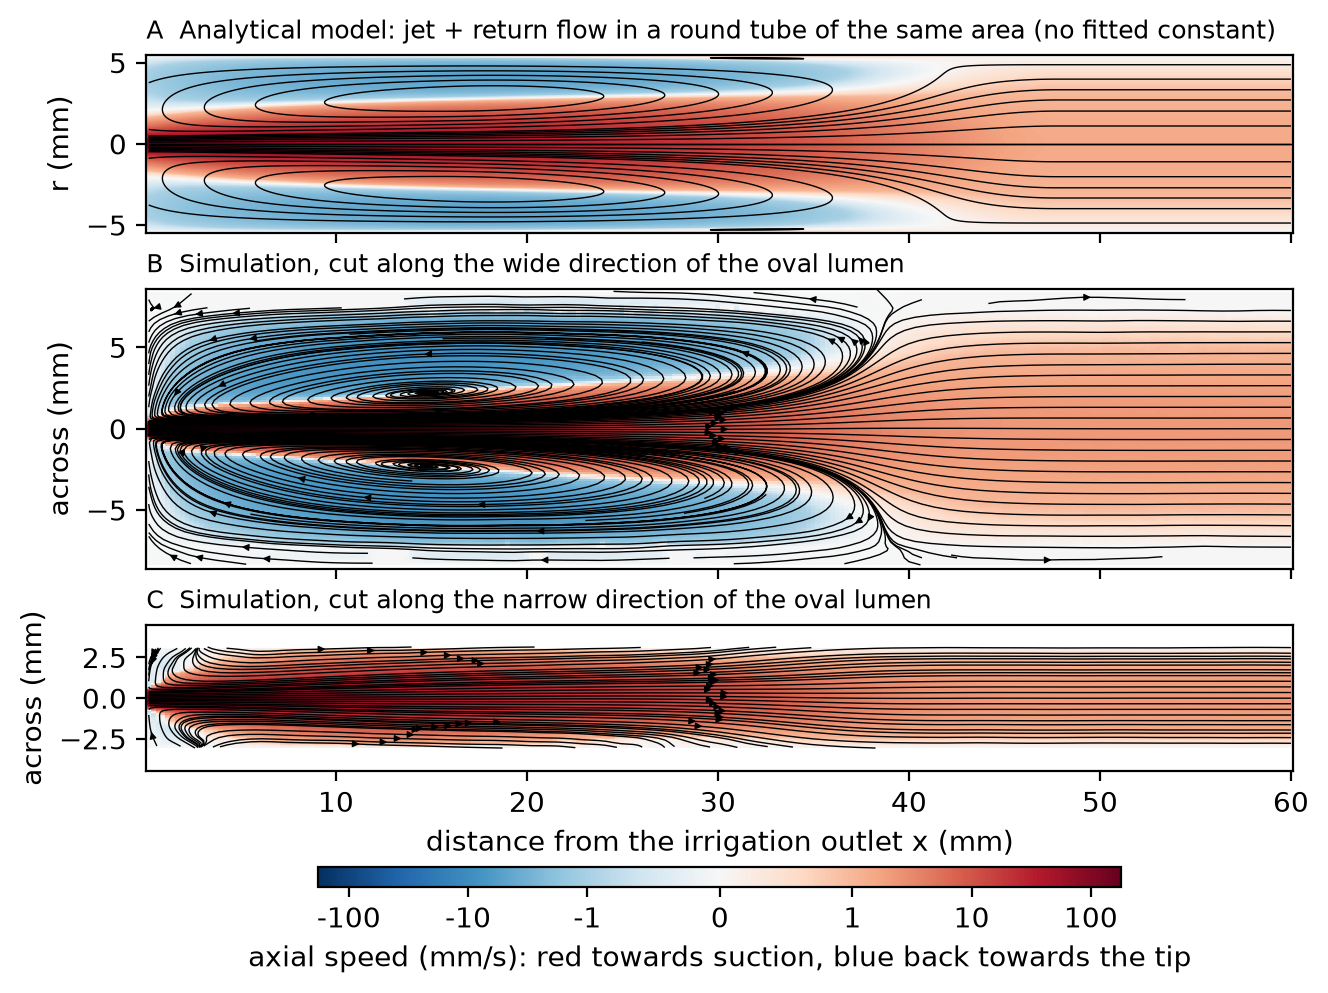
\includegraphics[width=0.9\linewidth]{fig_field.png}
\caption{Streamlines and axial speed. A: analytical model. B, C: simulation on the two mid-planes of the
oval lumen.}
\end{figure}
\begin{figure}[h]\centering
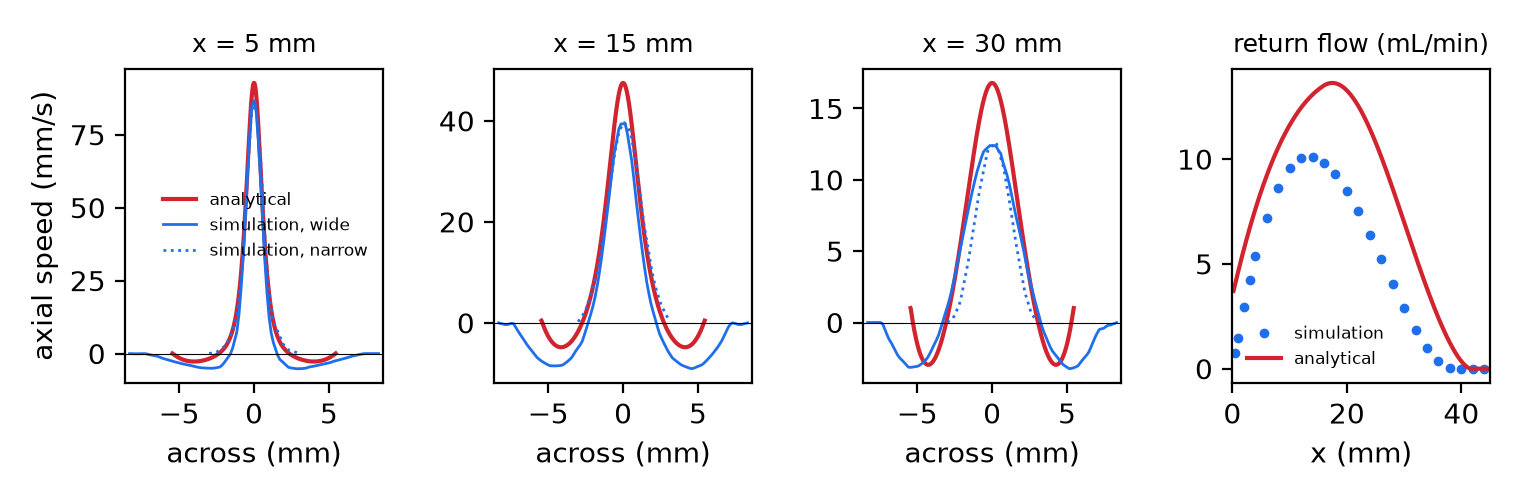
\includegraphics[width=\linewidth]{fig_profiles.png}
\caption{Axial speed across the lumen at three distances, and the return flow along the sheath.}
\end{figure}

What the model gets right: the ring vortex itself, its position, the jet profile and centre speed (within
15--30\,\% along the loop), the vortex centre at about $r=\SI{2.5}{mm}$, and the order of the return flow
(peak \SI{13.6}{mL/min} at \SI{17}{mm} against \SI{10.1}{mL/min} at \SI{14}{mm}).

What it misses: the lumen is oval, not round. In the simulation the fluid returns only through the two wide
sides of the oval; across the narrow direction the jet fills the height and everything moves forward (panel
C). The loop is therefore two lobes rather than a full ring, the return speed in the lobes is higher than
the model's, and the loop closes a little later (\SI{38}{mm} against \SI{32}{mm}). The model also starts
with a small return flow at $x=0$ because the idealised jet carries more than $Q$ at its virtual outlet.

\section{Pressure}\label{sec:p}
When the jet has spread over the lumen its momentum has become a pressure rise
\begin{equation}
\Delta p_{\rm jet}\simeq\frac{\rho K}{A}=\SI{0.09}{Pa}.
\end{equation}
The viscous loss of the duct flow is of the same small order: for a round tube of radius $R_{\rm eq}$ and
length \SI{80}{mm}, $\Delta p=8\mu LQ/\pi R_{\rm eq}^4=\SI{0.02}{Pa}$ (the ribs raise it; the simulation has
\SI{0.2}{Pa}). Both are negligible against the suction of \SI{933}{Pa} ($-7$ mmHg). The whole interior
sits at the suction pressure, and the flow pattern does not depend on the suction level: stronger suction
changes the pressure, not the flow, as long as the holes stay blocked.

\section{What it means for flushing}
\begin{figure}[h]\centering
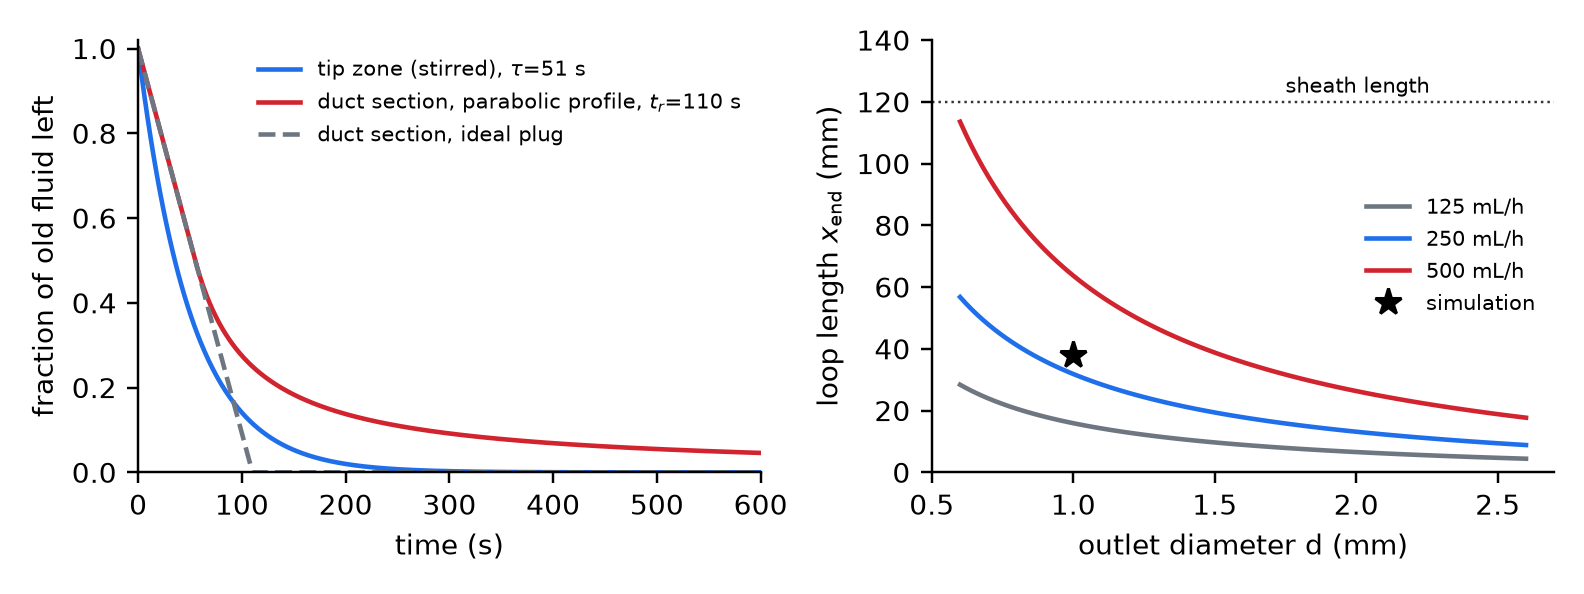
\includegraphics[width=0.95\linewidth]{fig_wash.png}
\caption{Left: fraction of old fluid left, tip zone and duct section taken separately. Right: loop length
from eq.~\eqref{eq:design} against outlet diameter for three irrigation rates; the star is the simulated
case.}
\end{figure}
\textbf{Tip zone (the loop).} Volume $V=A\,x_{\rm end}=\SI{3.5}{mL}$. The loop turns over in
$V/\max Q_{\rm back}\approx\SI{21}{s}$, faster than the through-flow time $\tau=V/Q=\SI{51}{s}$, so the
zone is roughly a stirred tank and old fluid leaves as
\begin{equation}
\phi_{\rm tip}(t)=e^{-t/\tau},\qquad \tau=\frac{A\,x_{\rm end}}{Q}=\SI{51}{s}.
\end{equation}
5\,\% is left after $3\tau\approx\SI{2.5}{min}$. Mixing is good, displacement is not: fresh irrigation is
diluted into the zone and part of it is carried round again.

\textbf{Duct section.} Length $L=\SI{82}{mm}$, mean residence $t_r=L/U_m=\SI{110}{s}$. Diffusion across
the lumen takes $R_{\rm eq}^2/D\approx\SI{3e4}{s}$ for $D=\SI{1e-9}{m^2/s}$, far longer, so each streamline
keeps its own speed. For a parabolic profile $u=2U_m(1-r^2/R^2)$ the fresh front has reached
$z=\min(L,ut)$, and integrating the remaining old fluid over the cross-section gives
\begin{equation}
\phi_{\rm duct}(t)=1-\frac{t}{t_r}\ \ \left(t\le\tfrac12t_r\right),\qquad
\phi_{\rm duct}(t)=\frac{t_r}{4t}\ \ \left(t\ge\tfrac12t_r\right).
\end{equation}
The centre is renewed after $t_r/2$, but the tail falls only as $1/t$: 8\,\% is still old after three
residence times (\SI{5.5}{min}). In the simulation the centre speed is \SI{2.2}{mm/s}, three times the
mean rather than two, because the ribs hold back the fluid near the wall. The first fresh fluid therefore
arrives sooner (simulated fastest transit \SI{42}{s}) and the tail is longer than this formula.

\textbf{Rib grooves.} The flow in the grooves is almost zero (23\,\% of the lumen volume moves at less than
a tenth of $U_m$). They are renewed mainly by diffusion: a groove \SI{1}{mm} deep needs of the order of
$w^2/D\approx\SI{1000}{s}$, about a quarter of an hour.

\section{Design consequences}
\begin{center}\begin{tabular}{rrrr}\toprule
Outlet $d$ (mm) & Outlet speed (mm/s) & $Re$ & Loop length, eq.~\eqref{eq:design} (mm)\\ \midrule
1.0 & 88 & 88 & 32 (simulation 38)\\
1.5 & 39 & 59 & 19\\
2.0 & 22 & 44 & 13\\
2.5 & 14 & 35 & 9\\ \bottomrule
\end{tabular}\end{center}
\begin{itemize}\setlength\itemsep{0pt}
\item A small outlet gives a long stirred zone at the tip, a large outlet gives a short one and more of
the sheath in plain displacement flow. Only the 1.0 mm row has been simulated.
\item Doubling the irrigation rate doubles the loop length and halves every flushing time.
\item Moving the outlet away from the tip leaves the fluid between the tip and the outlet with no
through-flow at all; it would be renewed only by whatever the loop stirs backwards. This is the question
for the planned position study.
\end{itemize}

\section{With some holes open: orifice estimate}
A side hole of area $A_h=\pi(\SI{0.5}{mm})^2$ under a pressure difference $\Delta p$ passes
\begin{equation}
Q_h=C_d\,A_h\sqrt{\frac{2\,\Delta p}{\rho}} .
\end{equation}
With the lumen about \SI{880}{Pa} below the outside this is $C_d\times\SI{62}{mL/min}$. The first open-hole
simulation (four holes near the tip, coarse mesh, first \SI{0.43}{s} only) gives \SI{38}{mL/min} per hole,
i.e.\ $C_d=0.61$, the usual value for a sharp orifice. Four open holes bring in about
\SI{152}{mL/min}, 36 times the irrigation.

Irrigation fluid can leave through a hole only if the lumen pressure exceeds the outside pressure. Carrying
the irrigation alone to the suction tube costs less than \SI{1}{Pa}, so the lumen stays close to the suction
pressure and the flow through every open hole is inward. Outflow through the holes requires the suction path
to be closed or the suction switched off. This part is preliminary until the open-hole runs are complete.

\section{Limits of this analysis}
Laminar, steady, single fluid; no tissue, air or clogging. The free-jet solution ignores the walls and is
used only where the jet is thin. The loop length carries the choice of ``edge'' of the jet and of the
equivalent radius. The simulated jet wobbles slightly (changes of 0.2\,\% per step remained), and the mesh
near the outlet resolves the \SI{1}{mm} jet with a limited number of cells, so simulation values near the
outlet are good to roughly 10\,\%.

\end{document}
